\chapter{ScatterPlot View}
\label{sec:scatter_view}

A ScatterPlot View displays the distribution of two numerical variables as points. When started, it presents itself in the following manner.

\begin{figure}[H]
    \hspace*{-2cm}
    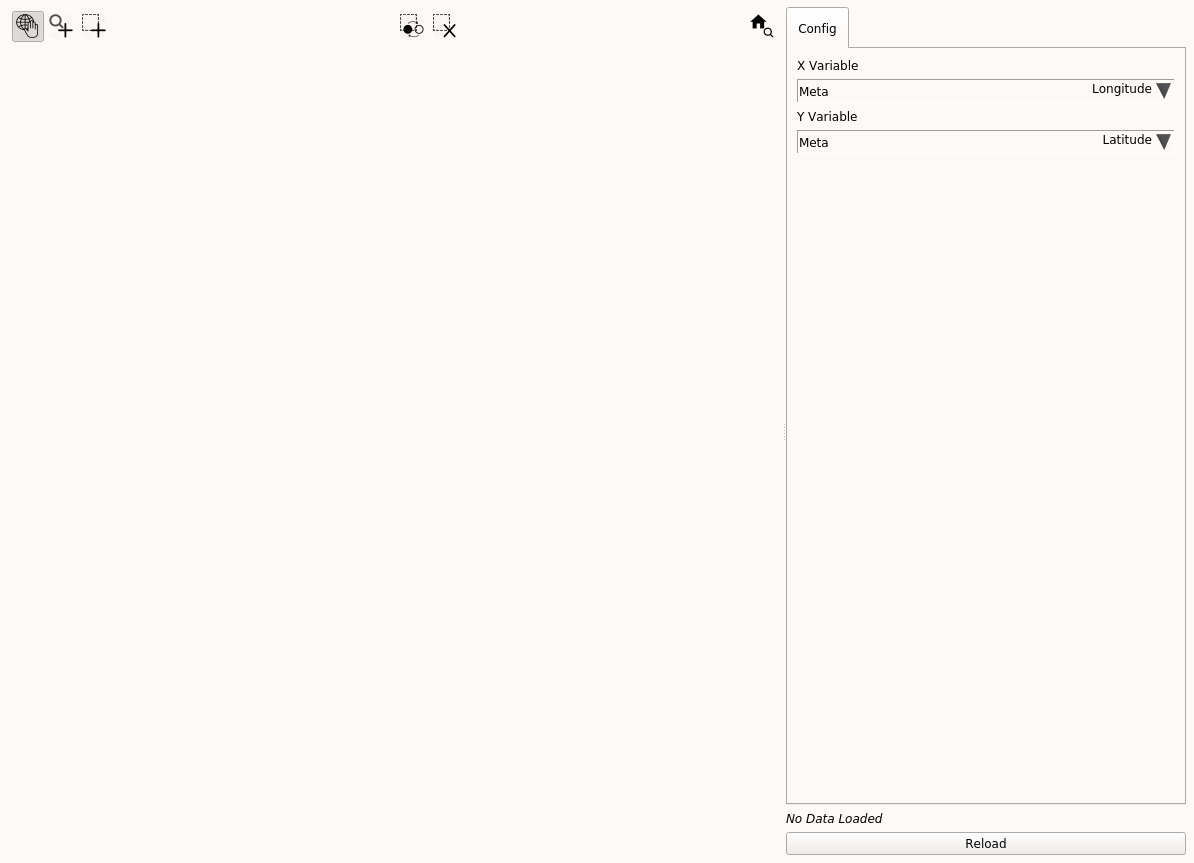
\includegraphics[width=18cm,frame]{figures/scatter_start.png}
  \caption{Scatterplot View startup}
\end{figure}

\section{Layout}

On the left side resides the plot area in which the data is visualized (if data has been loaded). The tool bar at the top shows the currently selected mouse interaction mode and the available actions.\\

On the right side resides the configuration area, which allows configuring what data is loaded and how it is displayed. The 'Reload' button on the bottom can be used to trigger a reload of the view's data.\\

Both areas can be resized and hidden if desired.

\section{Data Loading}

To load the data the mechanism described in Section \nameref{sec:ui_overview} or the 'Reload' button can be used. To filter the dataset, the mechanism described in Section \nameref{sec:filters} can be used. \\

\begin{figure}[H]
    \hspace*{-2cm}
    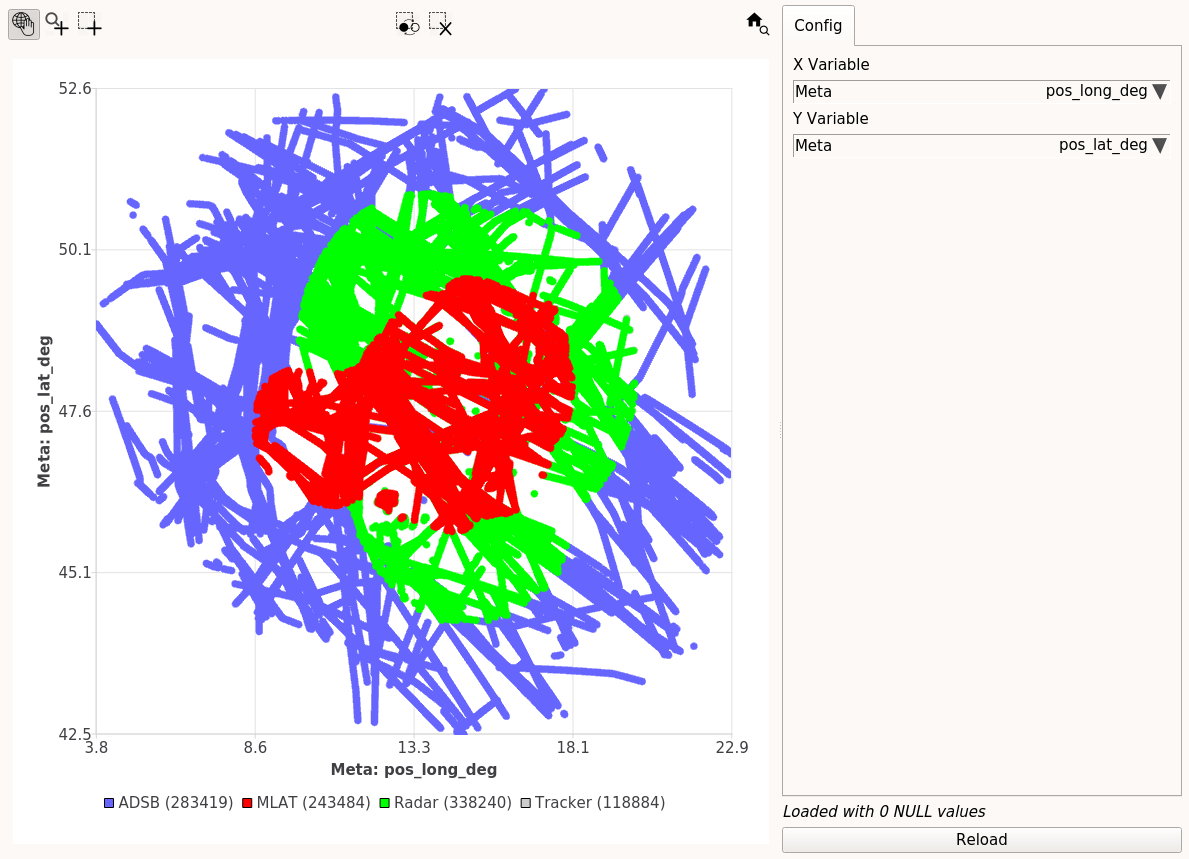
\includegraphics[width=18cm,frame]{figures/scatter_loaded.png}
  \caption{Scatterplot View after loading data}
\end{figure}

The values of the selected variables are used for positioning on the x-axis and y-axis. For each value pair a data point is generated. In the current example the WGS-84 meta-variables 'Longitude' and 'Latitude' are used, showing a similar view as the OSG View.
The color of each data point is defined by the DBContent it belongs to.\\

%TODO_V7 i think here it would be immensely important to tell the user why he might not see any data at all when selecting variables from two different DBContents!

On the bottom of the plot a legend is shown, giving the total counts of all data points.

\section{Usage}

\subsection{Toolbar}

The first tool buttons can be used to switch between the various mouse interaction modes:

\begin{table}[H]
  \center
  \begin{tabular}{ | l | l | l |}
    \hline
    \textbf{Icon} & \textbf{Text} &  \textbf{Description} \\ \hline
    \includegraphics[width=0.5cm,frame]{../../data/icons/navigate.png} & Navigate & Allows navigation of the data \\ \hline
    
\includegraphics[width=0.5cm,frame]{../../data/icons/zoom_select_action.png} & Zoom to Rectangle & Allows zooming to the selected rectangle \\ \hline
    
\includegraphics[width=0.5cm,frame]{../../data/icons/select_action.png} & Select & Allows data selection \& de-selection \\ \hline
  \end{tabular}
  \caption{Toolbar mouse interaction modes}
\end{table}

The others provide general actions by which the view can be modified (shortcut refers to keyboard shortcut):

%TODO_V7 Only refer to keyboard shortcuts when providing them

\begin{table}[H]
  \center
  \begin{tabular}{ | l | l | l | l |}
    \hline
    \textbf{Icon} & \textbf{Shortcut} &\textbf{Text} &  \textbf{Description} \\ \hline
    \includegraphics[width=0.5cm,frame]{../../data/icons/select_invert.png} & & Invert Selection & Selects all de-selected \& vice versa \\ \hline
    \includegraphics[width=0.5cm,frame]{../../data/icons/select_delete.png} & & Delete Selection & De-selects all target reports \\ \hline
    \includegraphics[width=0.5cm,frame]{../../data/icons/zoom_home.png} & & Zoom to Home & Pans/zooms to show all existing data \\ \hline
  \end{tabular}
  \caption{Toolbar actions}
\end{table} 

\subsection{Config Tab}

The selection controls on the top define which data variables are used to generate data points for the x/y-axis. Such a variable can be any numerical variable. A reload operation might be required for the selection to take effect. \\

Please note that visualization of evaluation result data is currently not implemented.

\subsection{Scatterplot}

\subsubsection{General Zoom}

The mouse wheel can be used to zoom in or out of the presented data, the space key can be used to reset to the default zoom level (euqivalent to \includegraphics[width=0.5cm,frame]{../../data/icons/zoom_home.png}).

\subsubsection{Navigation Mode}

In 'Navigate' mode, the left mouse-button can be used to pan the shown data.

\subsubsection{Zoom to Rectangle Mode}

In 'Zoom to Rectangle' mode, the left mouse-button can be used to select a rectangular region, to which a zoom operation is performed.

\subsubsection{Selection Mode}

In 'Select' mode, data can be selected. The first left mouse-button click starts selection (showing a red rectangle), the second click finalizes the selection. All data points inside the rectangular area are selected.

\begin{figure}[H]
    \hspace*{-2cm}
    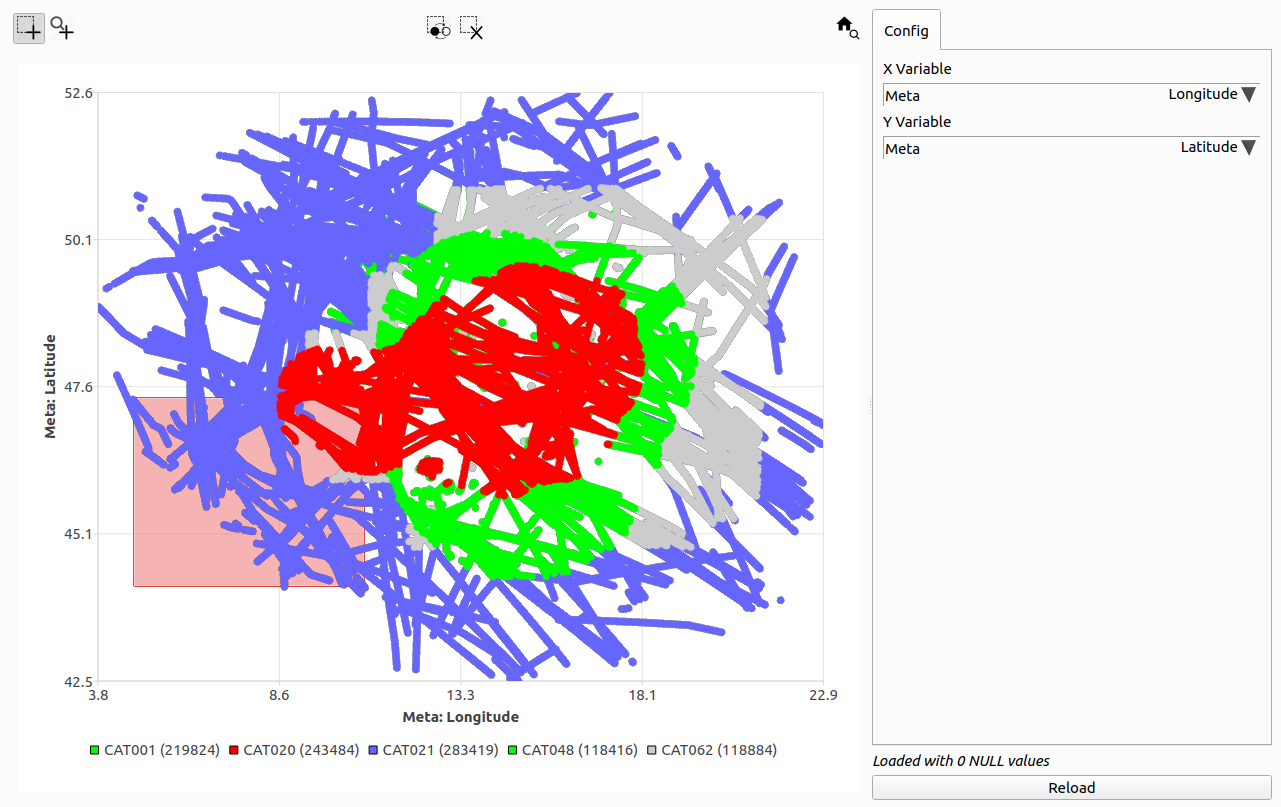
\includegraphics[width=18cm,frame]{figures/scatter_select.png}
  \caption{Scatterplot View data selection}
\end{figure}

The selected data is then presented in an extra 'Selected' entry in the legend, showing the count of all selected data points.

\begin{figure}[H]
    \hspace*{-2cm}
    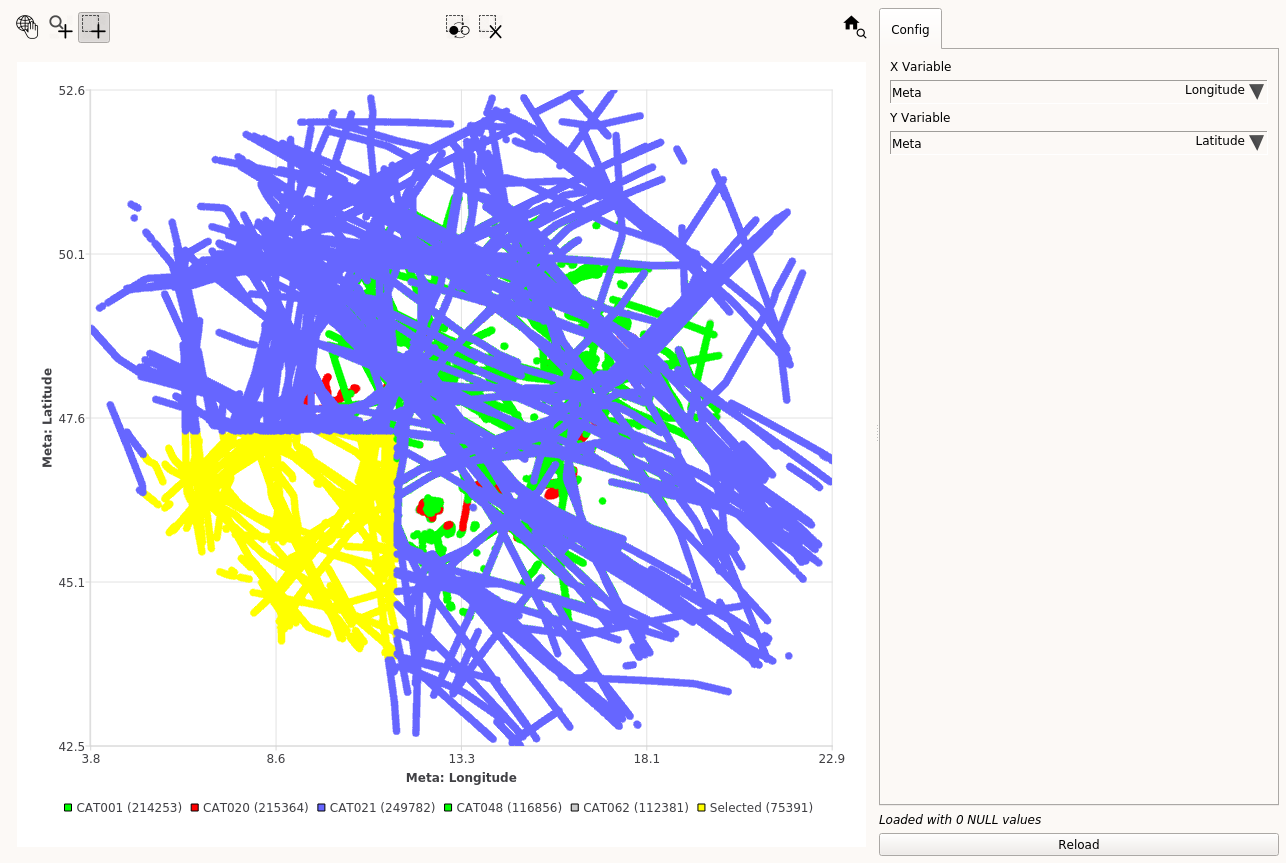
\includegraphics[width=18cm,frame]{figures/scatter_selected.png}
  \caption{Scatterplot View data selected}
\end{figure}

This enables selection of parts of the data based on the presented variables, allowing deeper analysis e.g. of dubious data. \\

%TODO_V7 maybe easier selection is the wrong term when talking about removing the selection?
%TODO_V7 lets discuss when we talk of 'points'/'data points' and 'target reports', this is mixed up a little at the moment
The 'Invert Selection' \includegraphics[width=0.5cm,frame]{../../data/icons/select_invert.png} or 'Delete Selection' \includegraphics[width=0.5cm,frame]{../../data/icons/select_delete.png} actions allow for easier selection of the wanted target reports. \\

By pressing the 'Control' key during the second click, the newly selected data is added to any previous selection. This can be used to select data incrementally, making more complex selections possible.
